\documentclass[a4paper, 12pt]{article}
\usepackage{listings} 
\usepackage{xcolor}
\usepackage{mdframed}
\usepackage{graphicx}
\usepackage{pgfplots}
\usepackage{float}
\usepackage{mathtools}

% Specific Line Breaks
% See https://tex.stackexchange.com/questions/26174/ for details
\usepackage[british]{babel} 

% Page Margins
\usepackage[margin=1.00in]{geometry}

% Large, array-sized, ceiling and floor operators
\DeclarePairedDelimiter\ceil{\lceil}{\rceil}
\DeclarePairedDelimiter\floor{\lfloor}{\rfloor}
\definecolor{code-gray}{gray}{0.93}

% Beginning of Document
\begin{document}
% Title
\title{ECE 443 - Project \#6}
\author{Collin Heist}
\date{\today}
\maketitle

% Table of Content and Listings
\pagenumbering{roman}
\tableofcontents
\newpage
\pagenumbering{arabic}

% Beginning of Report
\section{Design}
\label{sec:design}

I chose to partition my tasks by purpose. This ended up neatly partitioning the resources being used in this project, as well. In general, I decided to create the following tasks, each with the broad general purpose:

\begin{itemize}
\item \textbf{IO Reading Task} - Periodic task that reads from the temperature and motor speed buffer.
\item \textbf{RTR Sending Task} - Periodic task that sends an RTR request from CAN1 to CAN2.
\item \textbf{Change Notice Handler Task} - A really short task that processes presses of BTN1 into transitions between states of my control unit FSM.
\item \textbf{Control Unit Task} - A task that implements the functionality of the control unit as two \emph{states} of a finite state machine.
\item \textbf{PWM Updating Task} - A task that looks at the CAN2 RX channel for desired changes to the PWM output.
\end{itemize}

\section{IO Reading Task}
As described in the project outline, the IO Unit needed to periodically read the temperature and motor speeds, every 500 milliseconds. I chose to implement this as shown in \textbf{Listing~\ref{lst:task-read-IO}}.

	\begin{mdframed}[backgroundcolor=code-gray, roundcorner=10pt,
								innerleftmargin=5, innertopmargin=5, innerbottommargin=5]	
	\begin{lstlisting}[language=C, caption=IO Reading Task, tabsize=2, label={lst:task-read-IO}]
	static void task_read_IO(void* task_params) {
		float latest_temp, latest_rps;
		const TickType_t task_frequency= MS_TO_TICKS(IO_FREQ_MS);
		TickType_t last_time_awake = xTaskGetTickCount();
		for (;;) {
			latest_temp = read_ir_temp();
			latest_rps = get_average_rps();

			CAN2_refill_RTR_buffer(latest_temp, latest_rps,
				latest_pwm_setting);
		
			vTaskDelayUntil(&last_time_awake, task_frequency);
		}
	}
	\end{lstlisting}
	\end{mdframed}
	
This is a really simple task that on each iteration reads from the IR sensor and gets the average RPS values from my IR sensor and input capture libraries. Because the two \textit{units} should not communicate directly (that's what the CAN network is for), these variables are localized to this task. The exception to this is \textbf{latest\_pwm\_setting}, which is global. This is because this variable is changed inside the PWM updating task (see \textbf{Section~\ref{sec:pwm-updating-task}}). I could have used a queue to pass this data between these two tasks, or perhaps implemented the two tasks together, but I decided to treat the variable as 'private' (in a sense) and not permit any control unit code from accessing it.

The function, \textbf{CAN2\_refill\_RTR\_buffer()} is non-blocking and ensures that there is always one data frame inside the CAN2 TX channel. This function's code is shown here:

	\begin{mdframed}[backgroundcolor=code-gray, roundcorner=10pt,
								innerleftmargin=5, innertopmargin=5, innerbottommargin=5]	
	\begin{lstlisting}[language=C, caption=Refill CAN2 RTR Buffer Function, tabsize=2, label={lst:can2-refill-rtr-buffer}]
	void CAN2_refill_RTR_buffer(float temperature,
		float motor_speed, float pwm_setting) {
		
		CANTxMessageBuffer* message;

		if ((CANGetChannelEvent(CAN2, CAN_CHANNEL0) &
			 CAN_TX_CHANNEL_EMPTY) == 0)
			return;

		message = CANGetTxMessageBuffer(CAN2, CAN_CHANNEL0);

		// Clear the message values
		// Code omitted to save space
		
		// Format and create the RTR message itself
		// Code omitted to save space

		CANUpdateChannel(CAN2, CAN_CHANNEL0);
	}
	\end{lstlisting}
	\end{mdframed}
	
As you can see, I first check if the CAN2 TX channel is empty. If it is, that means that the CAN2 module has responded to an RTR  sent by CAN1. In this case, the buffer is first cleared (by assigning each \textbf{messageWord} field of the message structure to 0), and then the message is created. Without filling up an entire page, this sets the SID to the CAN2 RTR message ID, and sets the data-length code to 8.

The data itself is then partitioned into 8 sets of bytes. I chose to send a 10x scaled version of the temperature, and PWM setting, and a 100x scaled version of the motor speed. I did this in order to preserve the $\frac{1}{10}th$ place of each variable (and the $\frac{1}{100}th$ place for the motor speed), without taking up the entire 8 available bytes by sending a floating point value. This is achievable because even the 10x scaled values of these variables are well within the range of a \emph{short int} -- and for the 100x value of the motor speed, the data is sent across 4 bytes.

Because this function immediately returns if no new value is placed in the RTR TX channel, technically the individual RTR requests can be responded to with old data (up to 2 seconds old in the worst case). I went with this implementation because I found no way of (1) \emph{replacing} old values inside the RTR TX channel after they've been created, and (2) parsing more than one message from CAN1 (should the buffer just be added to), as each time the \textbf{CANUpdateChannel()} function is called, the buffer is cleared. In implementation, this is less of a problem than it sounds. Worst case, I could redesign the program to request data from the IO unit more often, and this would alleviate the problem.

This task is given a priority level of 3, with only the change-notice handler task being a higher priority. I chose this because reading from the IO units is important (and should take priority over the Control Unit FSM and PWM updating tasks), but takes very little time to execute and happens very infrequently -- alleviating the risk of taking away execution time of other tasks.

\section{RTR Sending Task}
\label{sec:rtr-sending-task}

This is by far the simplest task in my project. Once again, the project outline says that an RTR should be sent to the IO unit every 2000 milliseconds, so I implemented this as a periodic task with the only real `code' being the \textbf{CAN1\_send\_RTR()} function. The code for this task is shown in \textbf{Listing~\ref{lst:task-send-rtr}}.

	\begin{mdframed}[backgroundcolor=code-gray, roundcorner=10pt,
								innerleftmargin=5, innertopmargin=5, innerbottommargin=5]	
	\begin{lstlisting}[language=C, caption=RTR Sending Task, tabsize=2, label={lst:task-send-rtr}]
	static void task_send_RTR(void* task_params) {
		const TickType_t task_frequency = MS_TO_TICKS(RTR_FREQ_MS);
		TickType_t last_time_awake = xTaskGetTickCount();
		for (;;) {
			CAN1_send_RTR();
			LATBINV = LEDA;
		
			vTaskDelayUntil(&last_time_awake, task_frequency);
		}
	}
	\end{lstlisting}
	\end{mdframed}
	
Unblocking every \textbf{RTR\_FREQ\_MS} milliseconds (2000 as defined in the header), this just calls my CAN library function which sends and RTR from CAN1 to CAN2. 

This function is implemented at a task priority level of 3, the same as the IO reading task. I chose this priority level because it should only really be interrupted by the change-notice handler task, and it is fine to have the same priority level as the IO reading task -- as they're both very short-execution periodic tasks.

\section{Change Notice Handler Task}
\label{sec:change-notice-handler-task}

This task is exactly identical to previous projects. The change notice interrupt gives a semaphore to unblock this task, which then debounces the button. Upon a \textbf{button press} (as read by comparing the previous state of BTN1 to the current state of BTN1), the current global state of the Control Unit is toggled between configuration and operational mode. This task is the highest priority task in the project, as the responsiveness of the system is directly affected by this task's execution, and the execution time of this task is nearly negligible.

\section{Control Unit Task}
\label{sec:control-unit-task}

This is the first (and only) notably large task in this project. The entirety of the control-unit functionality (aside from sending RTR's to CAN2) is implemented in this task as a finite state machine. I will start with the state machine's declaration, and the code that executes every iteration of the task.

\subsection{Background FSM Code}

	\begin{mdframed}[backgroundcolor=code-gray, roundcorner=10pt,
								innerleftmargin=5, innertopmargin=5, innerbottommargin=5]	
	\begin{lstlisting}[language=C, caption=Control Unit Implementation, tabsize=2, label={lst:task-control-fsm-1}]
	enum STATE {CONFIGURATION_MODE, OPERATIONAL_MODE}
		current_state = CONFIGURATION_MODE;	
	
	static void task_control_FSM(void* task_params) {
		char top_lcd_str[18] = {'\0'};
		char bottom_lcd_str[18] = {'\0'};	
		float temp = 0, rps = 0, pwm = 0;
		float pwm_low_point = 0, pwm_high_point = 0;
		float desired_pwm = 0;
		unsigned int new_data_flag = FALSE;

		for (;;) {
			clear_string_buffer(top_lcd_str, sizeof(top_lcd_str));
			clear_string_buffer(bottom_lcd_str, sizeof(bottom_lcd_str));
		
			if (CAN1_process_RX(&temp, &rps, &pwm) ==
				CAN_MESSAGE_RECEIVED) {
				 
				LATBINV = LEDB;
				new_data_flag = TRUE;
			}

			switch (current_state) {
				case CONFIGURATION_MODE:
					// Code omitted 
					break;
				case OPERATIONAL_MODE:
					// Code omitted
					break;
			}

			taskYIELD();
		}
	}
	\end{lstlisting}
	\end{mdframed}
	
As typical in \textbf{C}, the FSM itself is implemented as an enum, and the machine is initialized to configuration mode (as outlined in the project description).

As for each loop of the task, it starts by clearing the two string buffers being utilized. I wrote the \textbf{clear\_string\_buffer} function to loop through all elements in the given character array and ensure each element is zero (the null character). This is done to prevent old messages from ending up on the LCD, and is important as these buffers are \emph{technically} static and are therefore never cleaned up on their own.

Afterwards, the RX channel of CAN1 is checked. This function returns\\ \textbf{CAN\_NO\_MESSAGE\_RECEIVED} if the RX channel was empty -- indicating that no RTR message has been sent or responded to. However, if it returns \\ \textbf{CAN\_MESSAGE\_RECEIVED}, then the three RTR variables (temperature, motor speed, and pwm setting) have their values updated based on the contents of the CAN1 RX channel. This event is noted by setting the new data flag to \textbf{TRUE}.

Next, the two states of the FSM are implemented (shown in \textbf{Listing~\ref{lst:task-control-fsm-2}} and \textbf{\ref{lst:task-control-fsm-3}}). And the task yields. This is important because this task's execution time can be quite long (with a lot of LCD functionality), and so other tasks should not be starved.

\subsection{Configuration Mode}
\label{subsec:configuration-mode}

Should the FSM currently be in \textbf{CONFIGURATION\_MODE}, then the following code will execute:

	\begin{mdframed}[backgroundcolor=code-gray, roundcorner=10pt,
								innerleftmargin=5, innertopmargin=5, innerbottommargin=5]	
	\begin{lstlisting}[language=C, caption=Control Unit - Configuration Mode, tabsize=2, label={lst:task-control-fsm-2}]
	case CONFIGURATION_MODE:
			LATGCLR = LED1;

			if (temp == 0)
				strcpy(top_lcd_str, BLANK_LINE);
			else
				sprintf(top_lcd_str, "	  %02.1f	  ", temp);

			set_cursor_LCD(FIRST_LINE_START);
			put_string_LCD(top_lcd_str);
			
			pwm_low_point = (PORTA & BTN3) ?
				temp : pwm_low_point;
			pwm_high_point = (PORTG & BTN2) ?
				temp : pwm_high_point;

			pwm_low_point = (pwm_high_point < pwm_low_point) ?
				0 : pwm_low_point;
			pwm_high_point = (pwm_high_point < pwm_low_point) ?
				0 : pwm_high_point;

			if (pwm_low_point == 0 && pwm_high_point == 0)
				strcpy(bottom_lcd_str, BLANK_LINE);
			else
				sprintf(bottom_lcd_str, "%02.1f		%02.1f",
					pwm_low_point, pwm_high_point);

			set_cursor_LCD(SECOND_LINE_START);
			put_string_LCD(bottom_lcd_str);
			break;
	\end{lstlisting}
	\end{mdframed}
	
The project outline gives descriptions as to how the top and bottom lines of the LCD should be displayed during this mode, and a majority of this function is simply manipulating the top and bottom LCD string accordingly. If button 2 or 3 are pressed during this task's execution, then the values for the PWM low and high point are set based off the current temperature.

This task has so many local variables because it explicitly cannot reference the global values of the temperature, motor speed, and PWM cycle -- as this would defeat the purpose of the CAN network. The most up-to-date values of the temperature (for this task) is obtained from the code shown in \textbf{Listing~\ref{lst:task-control-fsm-1}} that checks the CAN1 RX channel.

\subsection{Operational Mode}
\label{subsec:operational-mode}

Finally, if the unit is in \textbf{OPERATIONAL\_MODE}, then this code runs:

	\begin{mdframed}[backgroundcolor=code-gray, roundcorner=10pt,
								innerleftmargin=5, innertopmargin=5, innerbottommargin=5]	
	\begin{lstlisting}[language=C, caption=Control Unit - Operational Mode, tabsize=2, label={lst:task-control-fsm-3}]
	case OPERATIONAL_MODE:
		LATGSET = LED1;
	
		if (new_data_flag) {
			new_data_flag = FALSE;
			LATBINV = LEDB;
			sprintf(top_lcd_str, "%d%%	   %05.2f", (int)pwm, rps);
			sprintf(bottom_lcd_str, "%03.1f  %03.1f  %03.1f",
				pwm_low_point, temp, pwm_high_point);

			set_cursor_LCD(FIRST_LINE_START);
			put_string_LCD(top_lcd_str);
			set_cursor_LCD(SECOND_LINE_START);
			put_string_LCD(bottom_lcd_str);

			if (temp < pwm_low_point)
				desired_pwm = (float) PWM_MIN_VAL;
			else if (temp > pwm_high_point)
				desired_pwm = (float) PWM_MAX_VAL;
			else
				desired_pwm = (float)((PWM_LINEAR_MAX-PWM_LINEAR_MIN)*
					 (temp - pwm_low_point) /
					 (pwm_high_point - pwm_low_point) + PWM_LINEAR_MIN);

			CAN1_send_TX(desired_pwm);
			LATBINV = LEDC;
		}
		break;
	\end{lstlisting}
	\end{mdframed}
	
If no new data has been received since the last iteration of this task, nothing new needs to be done. However, if the CAN1 RX channel was not empty and the flag was set, then the LCD strings are reconstructed and displayed onto the screen. The only other functionality in this mode is to compute the newly desired PWM value, based off the current temperature (as well as the low and high set points), and send this data via CAN1 to CAN2.

The \textbf{CAN1\_send\_TX()} function is also quite simple, and sends the desired PWM setting as the 10x scaled value in order to preserve the $\frac{1}{10}th$ place. This is possible (once again) because the maximum value for the PWM is 100.0\%, and therefore can be represented by at most 1000 - well within the range of a \emph{short int}.

This task is given a priority of 2, lower than all other tasks except the PWM updating task. This is because all higher priority tasks are quicker to execute, and this task can be quite slow with all the LCD operations -- \emph{and} fast-response time from this task is not necessary.

\section{PWM Updating Task}
\label{sec:pwm-updating-task}

Finally, the PWM updating task is designed to be a non-periodic task that should ideally execute in round-robin style with the control unit task. They are both given a priority of 2, and yield at the end of their task's execution.

The code for this task is shown in \textbf{Listing~\ref{lst:task-update-pwm}}, below.

	\begin{mdframed}[backgroundcolor=code-gray, roundcorner=10pt,
								innerleftmargin=5, innertopmargin=5, innerbottommargin=5]	
	\begin{lstlisting}[language=C, caption=Control Unit - Operational Mode, tabsize=2, label={lst:task-control-fsm-3}]
	static void task_update_pwm(void* task_params) {
		for (;;) {
			if (CAN2_process_RX(&latest_pwm_setting) ==
				CAN_MESSAGE_RECEIVED) {
			
				if (set_pwm((unsigned int) latest_pwm_setting))
					// An error occurred
				else
					LATBINV = LEDD;
			}

			taskYIELD();
		}
	}
	\end{lstlisting}
	\end{mdframed}
	
Should the CAN2 RX channel be non-empty (indicating a new PWM setting is desired by the control unit), then that value is used to set the PWM module. In the event that the RX channel was empty, and no update to the PWM duty-cycle is desired, then this task shall immediately yield.

Here is where the global \textbf{latest\_pwm\_setting} variable is set, and a queue \emph{could} have been used to send this data directly to the IO reading task -- but as discussed before, this would add overhead and I simply avoided referencing the global variable inside the control unit functions to appropriately partition my two units.
	
%\begin{figure}[H]
%\centering
%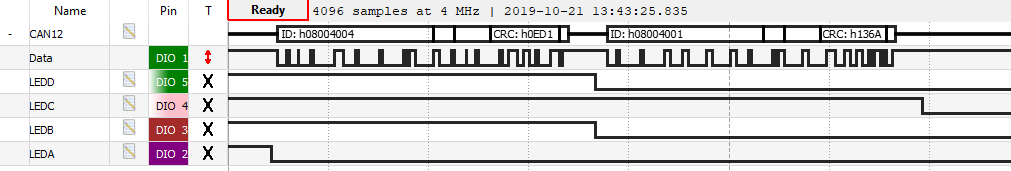
\includegraphics[width=\textwidth]{fig-can-buttons.PNG}
%\caption{WaveForms capture of the CAN message and LED's}
%\label{fig:can-buttons}
%\end{figure}

\end{document}